\documentclass{article}

\usepackage[margin=2.5cm,left=2cm,includefoot]{geometry}
\usepackage{graphicx}
\usepackage{float}
\usepackage[space]{grffile}
\usepackage{hyperref}
\usepackage[export]{adjustbox}
\usepackage{multicol}
\usepackage{caption}
\usepackage{hyperref}
\usepackage{listings}
\usepackage{vhistory}
\newcommand{\nexists}{\not\exists}
\newcommand\tab[1][0.5cm]{\hspace*{#1}}

% Header and footer
\usepackage{fancyhdr}
\pagestyle{fancy}

\rhead{COS301}
\lhead{Functional Specification}
\fancyfoot[R]{Page \thepage}

\renewcommand{\headrulewidth}{2pt}
\renewcommand{\footrulewidth}{1pt}

\begin{document}

	\begin{titlepage}
		\begin{center}
			
\includegraphics[width=10cm]{images/marketlead_3.png}  \\
			[0.5cm]
			\huge{
			Functional Specification\\
			}

			\line(1,0){300}\\
			[0.2cm]
			\LARGE{Project: Insurance profiling from social media\\
			Client: RetroRabbit} \\
			\line(1,0){300}\\
			\LARGE{Team: Valknut Solutions}\\
			[1.0cm]
			\large{Version: 1.3}\\
			\large
			{
			\begin{itemize}
				\item 13054903 - Charl Jansen van Vuuren
				\item 13044924 - Kevin Heritage
				\item 13176545 - Quinton Weenink\\
			\end{itemize}
			}
			\textsc{\large}\\
		[1.0cm]
		\textsc{\large  Department of Computer Science}\\
		[0.5cm]
		\textsc{\large \today}\\
		\end{center}

		%\begin{figure}[H]}
		%\centering
		%\includegraphics[{imagename}
		%\end{figure}\

	\end{titlepage}
	\cleardoublepage
	\tableofcontents
	\cleardoublepage
	% Start of the revision history table
	\begin{versionhistory}
  		\vhEntry{1.0}{27.05.2016}{CJvV,KH,QW}{Original Architectural document without Functional requirements}
  		\vhEntry{1.1}{27.07.2016}{CJvV,KH,QW}{Added Functional requirements and separated Architectural requirements}
		\vhEntry{1.2}{09.09.2016}{CJvV,KH,QW}{Added better scoping requirements, updated use cases, updated each subsystem, added descriptions to each section}
		\vhEntry{1.3}{05.11.2016}{CJvV,KH,QW}{Added logo,Marketing use cases, marketing activity diagram, updated some styling and added service contract specification for marketing case}
	\end{versionhistory}
	
	\pagebreak


\section{Functional requirements and application design}
This document is related to the design requirements related to the Insurance profiling project, for a more thorough overview of the system see the Architectural Specification's scope and overview.
\subsection{Document overview}
The functional requirement specification of this system is separated into different sections, namely:
\begin{itemize}
	\item The overall scope of the system from a high level stand point
	\item The smaller subsystems of the high level scope including
		\begin{enumerate}
			\item A use case diagram of that subsystem
			\item A service contract 
			\item The required functionality for that use case
			\item A process specification if the use case functionality is complex
		\end{enumerate}
	\item Domain models based on the use cases - See Section \ref{sec:domain}
	\item Any related open issues - See Section \ref{sec:open}
\end{itemize}
	\subsection{Overall System Scope}
	The system consists of five modularized subsystems namely:
	\begin{itemize}
		\item Administration Section \ref{subsec:Admin}
		\item Notifications Section \ref{subsec:Notifcations}
		\item Analysis Section \ref{subsec:Analysis}
		\item Persistence with regards to data Section \ref{subsec:Persistence}
		\item Social media Section \ref{subsec:SocialMedia}
	\end{itemize}
		\begin{figure}[H]
		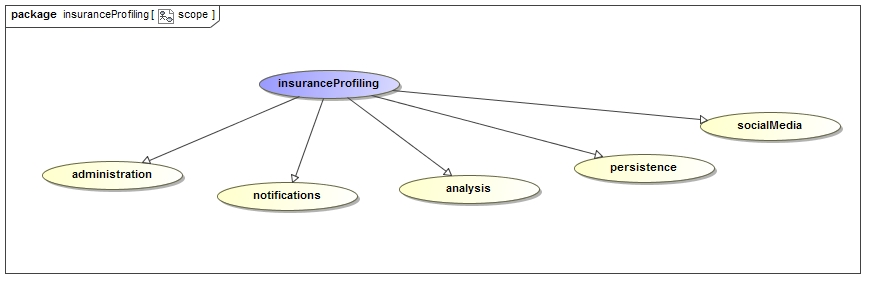
\includegraphics[width=\textwidth]{images/uc__insuranceProfiling__scope.jpg}  \\
		\caption{Scope : Insurance Profiling}
		\end{figure}
		
		
		\pagebreak
	\subsection{Social Media subsystem}\label{subsec:SocialMedia}
	The social media subsystem forms a major part of the system's functionality. \\The included modules handle the receiving of data from the Facebook advertisement lead form, the Wechat messenger bot and the Facebook messenger. The social media aspect further includes the website's lead form integration point.\\
		\subsubsection{Use cases}
		\begin{figure}[H]
		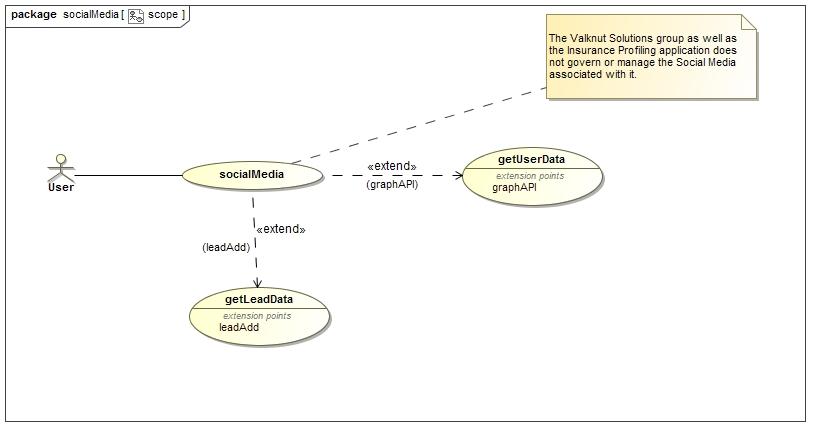
\includegraphics[width=\textwidth]{images/uc__socialMedia__scope.jpg}  \\
		\caption{Use Case Diagram : Social Media}
		\end{figure}

		\begin{flushleft}
			\textbf{Critical}
				\begin{itemize}
	  				\item validateCustomer
	  				\item createCustomer
	  				\item getCustomer
				\end{itemize}
			\textbf{Important}
				\begin{itemize}
	  				\item validateCustomer
				\end{itemize}
			\textbf{Nice-To-Have}
				\begin{itemize}
	  				\item getAnalyst
	  				\item analyseUser
				\end{itemize}
		\end{flushleft}

		\subsubsection{Services Contracts}
		\begin{itemize}
			\item Pre-conditions
				\begin{itemize}
					\item The information is valid
				\end{itemize}
			\item Post-conditions
				\begin{itemize}
					\item The user's information will be saved in the database
					\item A new lead will be created in the database to follow up on
				\end{itemize}
		\end{itemize}
		\begin{figure}[H]
		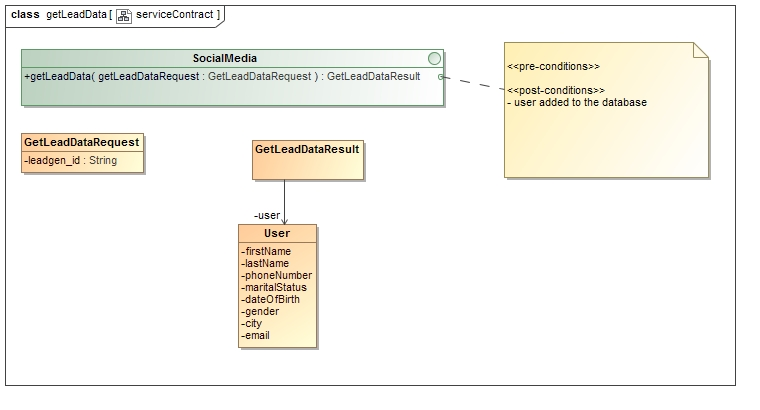
\includegraphics[width=\textwidth]{images/class__getLeadData__serviceContract.jpg}  \\
		\caption{Service Contract : getLeadData}
		\end{figure}

		\subsubsection{Required Functionality}

		\begin{figure}[H]
		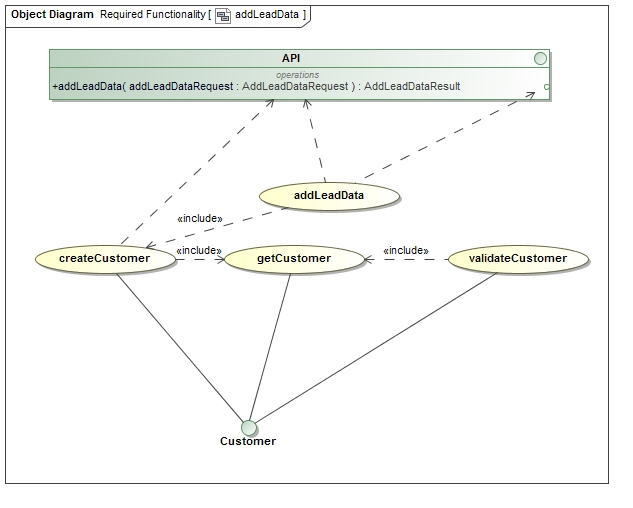
\includegraphics[width=\textwidth]{images/obj__Required_Functionality__addLeadData.jpg}  \\
		\caption{Required Functionality : getLeadData}
		\end{figure}

		%\subsubsection{Process specifications}
		%\begin{figure}[H]
		%
\includegraphics[width=\textwidth]{images/Incomplete.png}  \\
		%\caption{Process specification : getLeadData}
		%\end{figure}
		
	\pagebreak
	\subsection{Analysis subsystem}\label{subsec:Analysis}
	The analysis subsystem handles another core functionality of the system, analysis of the retrieved data.\\ This includes the ability to generate reports in the form of different graphs, filtered by different fields.\\ Analysis and reporting forms a major feature from a marketing and risk analysis standpoint.
		\subsubsection{Use cases}

		\begin{figure}[H]
		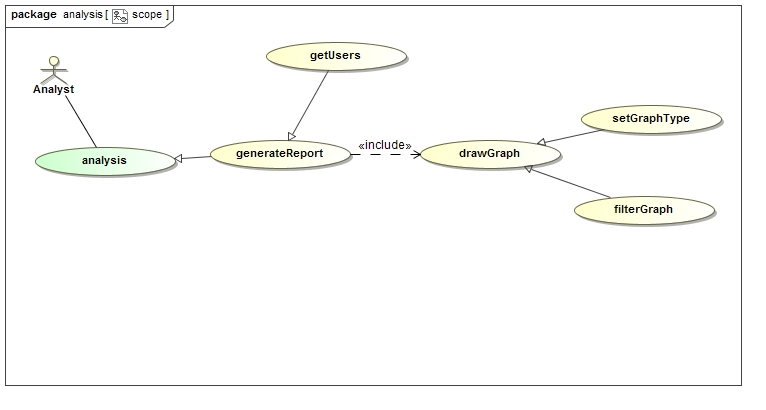
\includegraphics[width=\textwidth]{images/uc__analysis__scope.jpg}  \\
		\caption{Use Case Diagram : Analysis}
		\end{figure}

		\begin{flushleft}
			\textbf{Critical}
				\begin{itemize}
					\item getUsers
					\item generateReport
					\item drawGraph
				\end{itemize}
			\textbf{Important}
				\begin{itemize}
				\item setGraphType
					\begin{itemize}
						\item Pie graph
						\item Bar graph
						\item Line graph
					\end{itemize}
				\end{itemize}

			\textbf{Nice-To-Have}
				\begin{itemize}
					\item filterGraph - Including:
					\begin{itemize}
						\item Gender
						\item Age
						\item Location
						\item Marital status
						\item The amount of signups per year
					\end{itemize}
				\end{itemize}
		\end{flushleft}
		\subsubsection{Services Contracts}
		\begin{itemize}
			\item Pre-conditions
				\begin{itemize}
					\item The analyst is logged in
					\item The analyst must choose the graph data to filter by
					\item The analyst must choose the graph type to generate
				\end{itemize}
			\item Post-conditions
				\begin{itemize}
					\item A report is generated. This report includes
						\begin{itemize}
							\item The graph types the analyst chose
							\item The graph data the analyst chose 
						\end{itemize}
				\end{itemize}
		\end{itemize}
		\begin{figure}[H]
		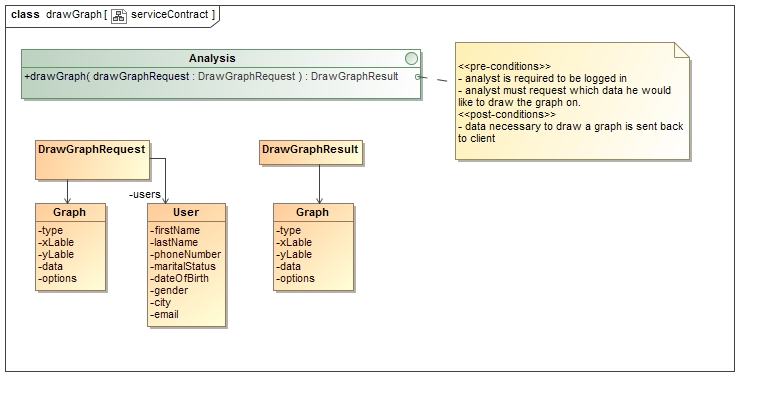
\includegraphics[width=\textwidth]{images/class__drawGraph__serviceContract.jpg}  \\
		\caption{Service Contract : generateReport}
		\end{figure}

		%\subsubsection{Required Functionality}
		%\begin{figure}[H]
		%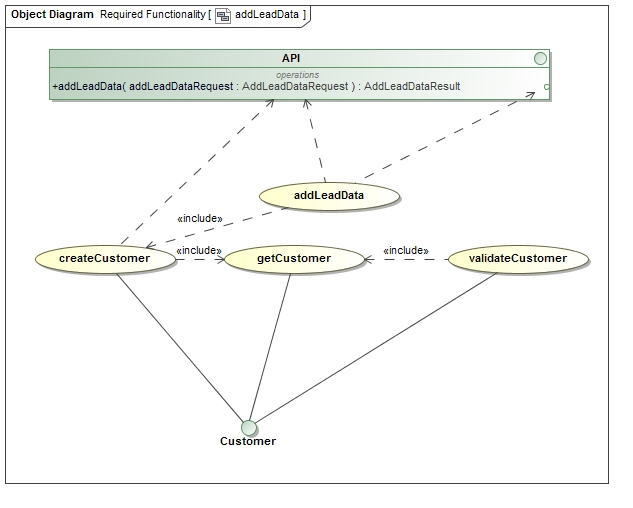
\includegraphics[width=\textwidth]{images/obj__Required_Functionality__addLeadData.jpg}  \\
		%\caption{Required Functionality : drawGraph}
		%\end{figure}

		\subsubsection{Process specifications}
		\begin{figure}[H]
		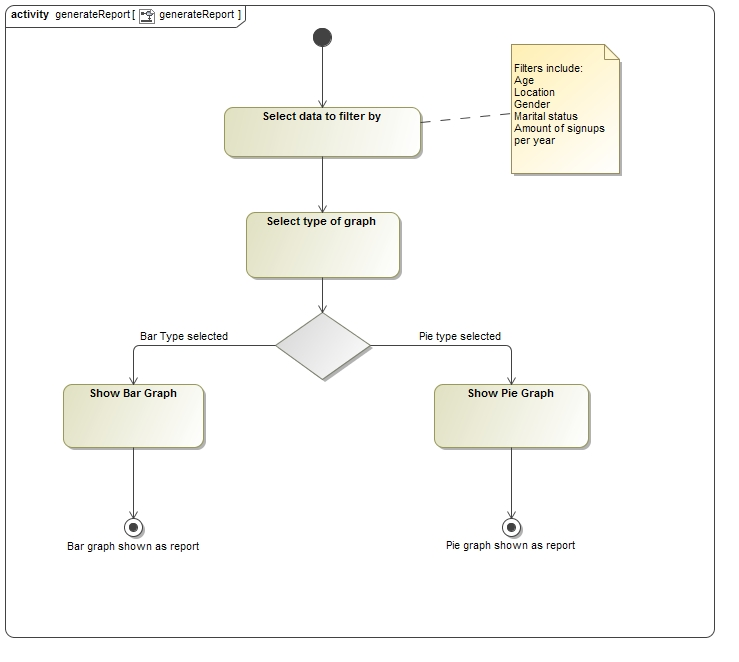
\includegraphics[width=\textwidth]{images/process__generateReport.jpg}  \\
		\caption{Process specification : generateReport}
		\end{figure}
	\pagebreak
	\subsection{Administration subsystem}\label{subsec:Admin}
	The administration subsystem handles the authentication and management of the analysts and administrators of the system.
		\subsubsection{Use cases}
		\begin{figure}[H]
		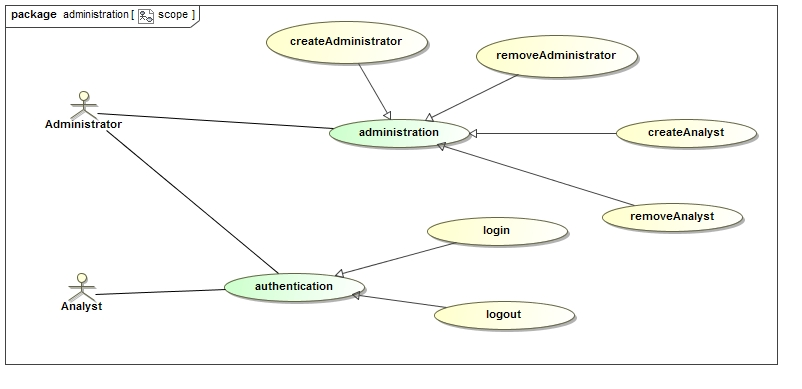
\includegraphics[width=\textwidth]{images/uc__administration__scope.jpg}  \\
		\caption{Use Case Diagram : Administration}
		\end{figure}

		\begin{flushleft}
			\textbf{Critical}
				\begin{itemize}
					\item createAdministrator
					\item createAnalyst
					\item login
					\item getUser
				\end{itemize}
			\textbf{Important}
				\begin{itemize}
					\item removeAnalyst
					\item removeAdministrator
				\end{itemize}

			\textbf{Nice-To-Have}
				\begin{itemize}
					\item logout
					\item analyseUser
				\end{itemize}
		\end{flushleft}

		\subsubsection{Services Contracts}
		\begin{itemize}
			\item Pre-conditions
				\begin{itemize}
					\item The admin is logged in Figure \ref{fig:createAdmin}
					\item An analyst is logged in Figure \ref{fig:authentication}
					\item A valid request is made
				\end{itemize}
			\item Post-conditions
				\begin{itemize}
					\item The analyst receives the results of the valid request
				\end{itemize}
		\end{itemize}
		\begin{figure}[H]
		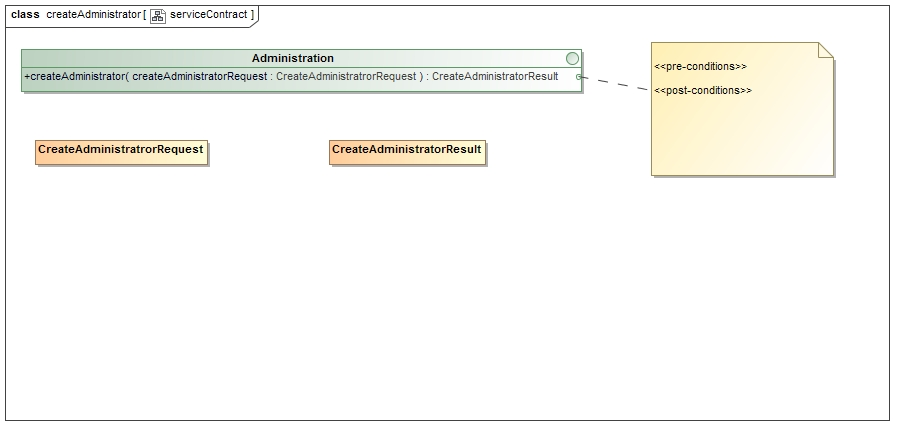
\includegraphics[width=\textwidth]{images/class__createAdministrator__serviceContract.jpg}  \\
		\caption{Service Contract : createAdministrator}
		\label{fig:createAdmin}
		\end{figure}
		
		\pagebreak
	\subsubsection{Authentication module}\label{subsubsec:Auth}		
	The authentication module, as part of the higher level Adminstrator subsystem, handles the identification and access control of Analysts. An analyst must login before any features available to them are available.
		\begin{figure}[H]
		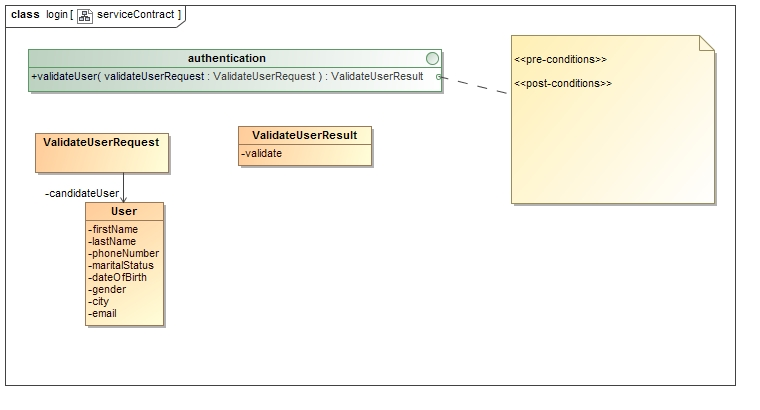
\includegraphics[width=\textwidth]{images/class__login__serviceContract.jpg}  \\
		\caption{Service Contract : Authentication}
		\label{fig:authentication}
		\end{figure}
		
		
	\pagebreak
		
\subsection{Marketing subsystem}\label{subsec:marketing}
	The Marketing subsystem handles the ability to process new user leads.\\ This includes updating user's information and marking the user as processed. Uninterested users can decline the processing, removing that user's information.
		\subsubsection{Use cases}
		\begin{figure}[H]
		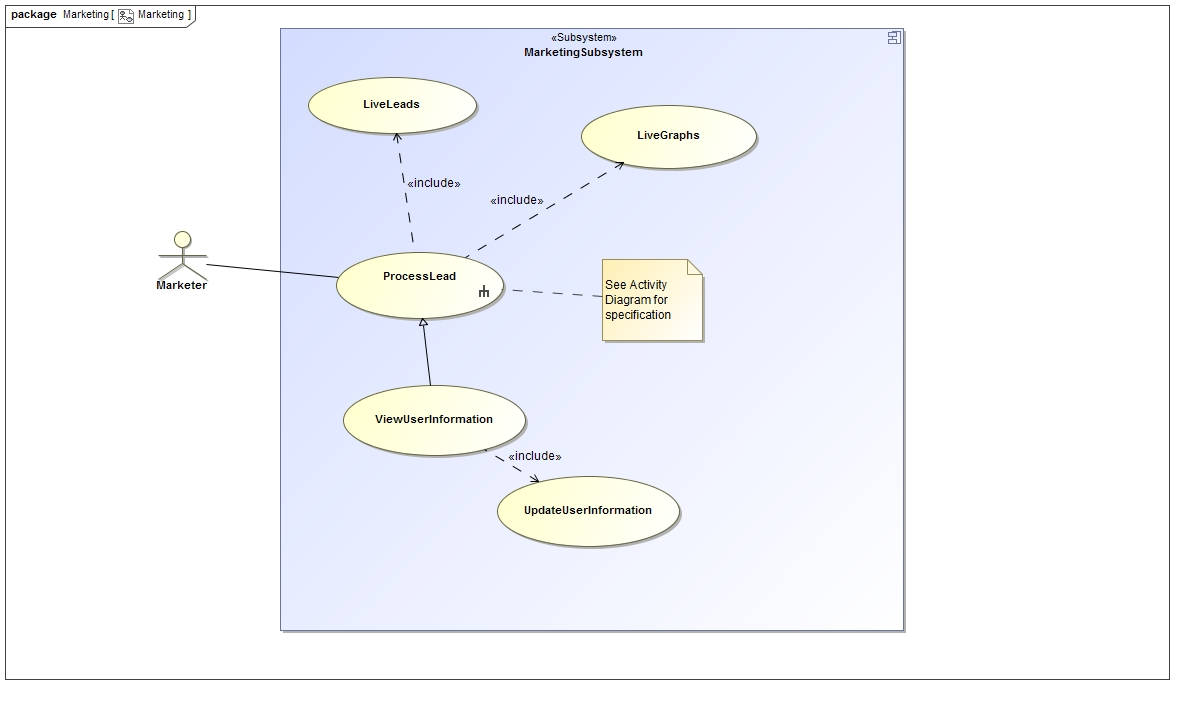
\includegraphics[width=\textwidth]{images/uc__marketing_scope.jpg}  \\
		\caption{Use Case Diagram : Marketing}
		\end{figure}

		\begin{flushleft}
			\textbf{Critical}
				\begin{itemize}
					\item ProcessLead
					\item ViewUserInformation
				\end{itemize}
			\textbf{Important}
				\begin{itemize}
					\item LiveLeads
					\item UpdateUserInformation
				\end{itemize}
			\textbf{Nice-to-have}
				\begin{itemize}
					\item LiveGraphs
				\end{itemize}
		\end{flushleft}

		\subsubsection{Services Contracts}
		The pre and post conditions for the marketing processing of a lead is described below:
		\begin{itemize}
				\item Pre-conditions
				\begin{itemize}
					\item The marketer is logged in.
					\item A user lead is created (from any integration)
				\end{itemize}
			\item Post-conditions
				\begin{itemize}
					\item The marketer processes the lead. See Figure \ref{fig:processLead} for more information.
				\end{itemize}
		\end{itemize}

		
		\subsubsection{Process specifications}
		\begin{figure}[H]
		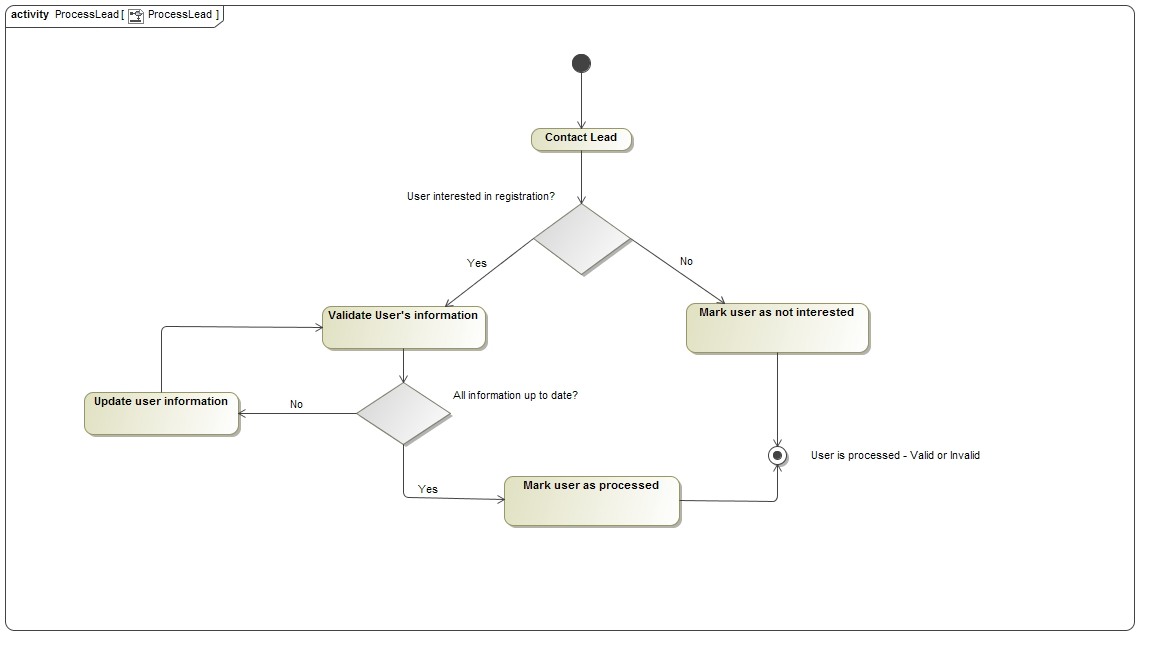
\includegraphics[width=18cm]{images/marketingProcess.jpg}  \\
		\caption{Process specification : ProcessLead}
		\label{fig:processLead}
		\end{figure}

		

		%\subsubsection{Required Functionality}

		%\begin{figure}[H]
		%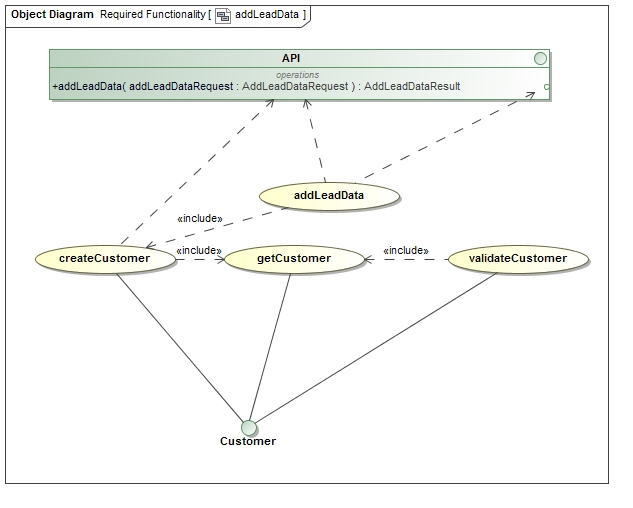
\includegraphics[width=\textwidth]{images/obj__Required_Functionality__addLeadData.jpg}  \\
		%\caption{Required Functionality : notify}
		%\end{figure}

		%\subsubsection{Process specifications}

		%\begin{figure}[H]
		%
\includegraphics[width=\textwidth]{images/Incomplete.png}  \\
		%\caption{Process specification : notify}
		%\end{figure}
		
		
		

		%\subsubsection{Required Functionality}

		%\begin{figure}[H]
		%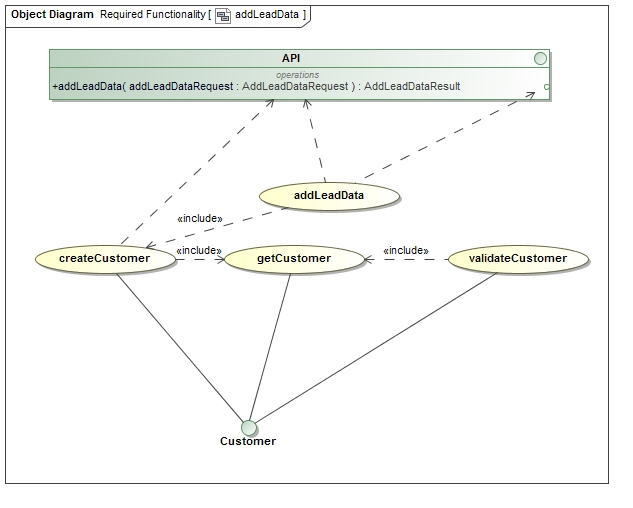
\includegraphics[width=\textwidth]{images/obj__Required_Functionality__addLeadData.jpg}  \\
		%\caption{Required Functionality : createAdministrator}
		%\end{figure}

		%\subsubsection{Process specifications}

		%\begin{figure}[H]
		%
\includegraphics[width=\textwidth]{images/Incomplete.png}  \\
		%\caption{Process specification : createAdministrator}
		%\end{figure}

	\pagebreak
	\subsection{Persistence subsystem}\label{subsec:Persistence}
	The persistence subsystem handles the throughout persisting of information in the system. \\Persistence in this case related to the information passing between database and system. \\ Users, analysts and Adminstrators data are all persisted throughout the system. \\ This ensures any changes to a user, analyst or admin's data, is synchronized with the database system.
		\subsubsection{Use cases}

		\begin{figure}[H]
		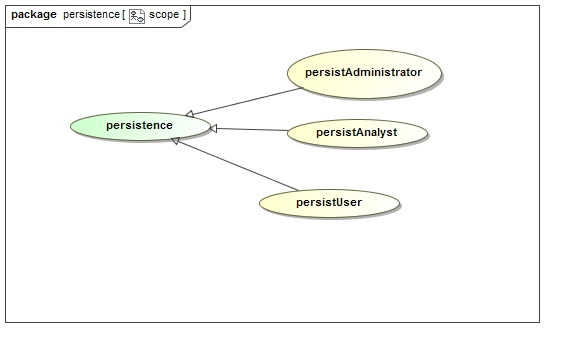
\includegraphics[width=\textwidth]{images/uc__persistence__scope.jpg}  \\
		\caption{Use Case Diagram : Persistence}
		\end{figure}

		\begin{flushleft}
			\textbf{Critical}
				\begin{itemize}
					\item persistAdministrator
					\item persistAnalyst
					\item persistUser
				\end{itemize}
		\end{flushleft}

		%\subsubsection{Services Contracts}

		%\begin{figure}[H]
		%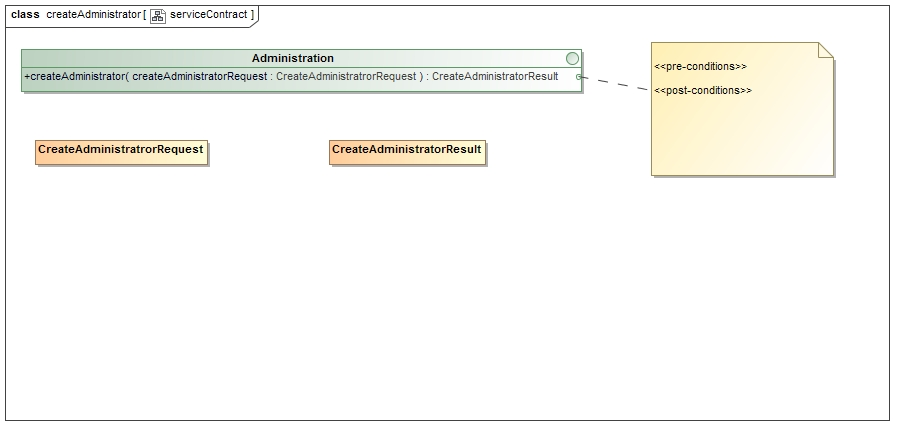
\includegraphics[width=\textwidth]{images/class__createAdministrator__serviceContract.jpg}  \\
		%\caption{Service Contract : persistUser}
		%\end{figure}

		%\subsubsection{Required Functionality}

		%\begin{figure}[H]
		%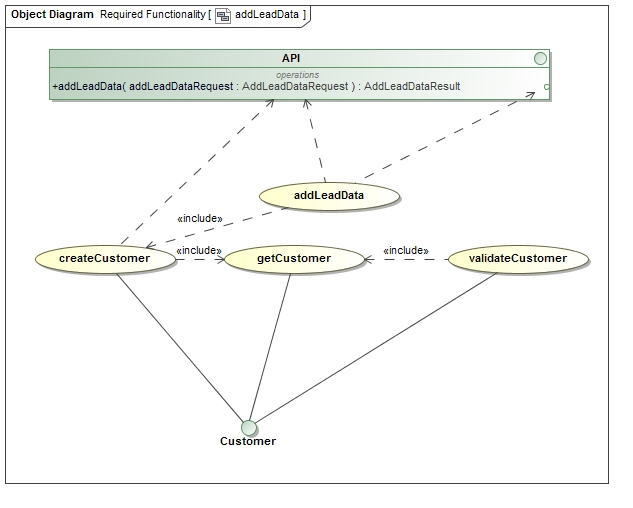
\includegraphics[width=\textwidth]{images/obj__Required_Functionality__addLeadData.jpg}  \\
		%\caption{Required Functionality : persistUser}
		%\end{figure}

		%\subsubsection{Process specifications}

		%\begin{figure}[H]
		%
\includegraphics[width=\textwidth]{images/Incomplete.png}  \\
		%\caption{Process specification : persistUser}
		%\end{figure}

	\pagebreak
	\subsection{Notifications subsystem}\label{subsec:Notifcations}
	The notification subsystem handles the ability to send responses to customers and analysts.\\ The use case might seem simplified, but this design allows for different notification channels. \\The notify module can be specialized in the format of Email, SMS and JSON responses or any other accessible notification module.
		\subsubsection{Use cases}
		
		\begin{figure}[H]
		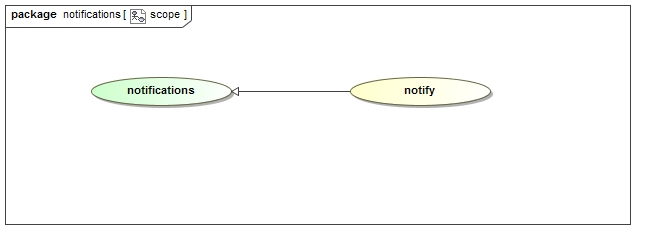
\includegraphics[width=\textwidth]{images/uc__notifications__scope.jpg}  \\
		\caption{Use Case Diagram : Notifications}
		\end{figure}

		\begin{flushleft}
			\textbf{Critical}
				\begin{itemize}
					\item Notify
				\end{itemize}
			\textbf{Important}
				\begin{itemize}
					\item Email
				\end{itemize}
			\textbf{Nice-to-have}
				\begin{itemize}
					\item SMS
					\item JSON Objects
				\end{itemize}
		\end{flushleft}

		\subsubsection{Services Contracts}
			\begin{itemize}
			\item Pre-conditions
				\begin{itemize}
					\item The sender's notification point is valid
					\item The recipient's notification point is valid
					\item eg. Valid email addresses
				\end{itemize}
			\item Post-conditions
				\begin{itemize}
					\item A success message will be received 
				\end{itemize}
		\end{itemize}
		\begin{figure}[H]
		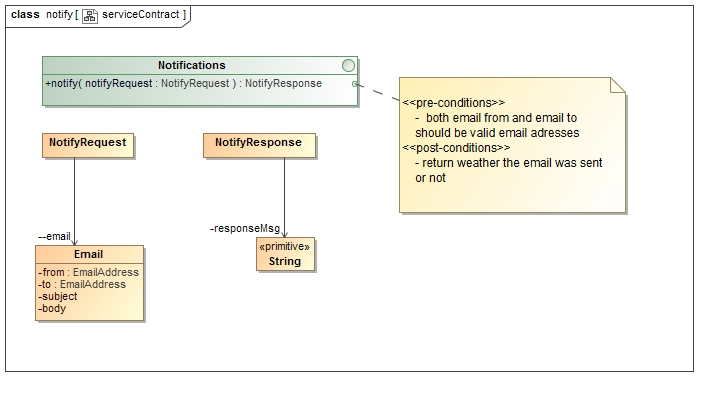
\includegraphics[width=\textwidth]{images/class__notify__serviceContract.jpg}  \\
		\caption{Service Contract : notify}
		\end{figure}
		
		
		
		


\pagebreak
\subsection{Domain model}\label{sec:domain}
The domain model shows the objects, their attributes and the relationships between these objects. \\
The included domain models specify the Analysis model Figure \ref{fig:domain_admin} and the LeadAd/User model Figure \ref{fig:domain_user}.
\begin{figure}[H]
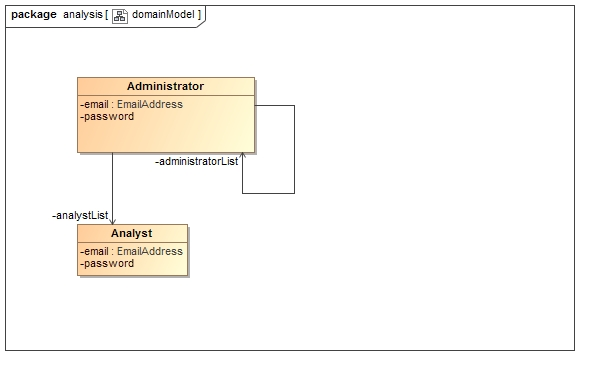
\includegraphics[width=\textwidth]{images/class__analysis__domainModel.jpg}  \\
\caption{Domain Model : Analysis}
\label{fig:domain_admin}
\end{figure}

\begin{figure}[H]
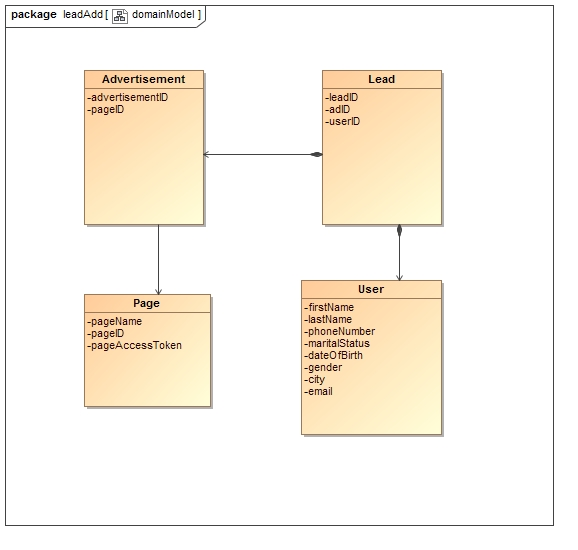
\includegraphics[width=\textwidth]{images/class__leadAdd__domainModel.jpg}  \\
\caption{Domain Model : Social Media}
\label{fig:domain_user}
\end{figure}


\subsection{Open Issues}\label{sec:open}
At the current version of  the system, all the requirements are addressed and all previous issues were clarified by our client.





\end{document}
